\documentclass[16pt]{extarticle}

%opening
\title{Second Work-in-Progress}
\author{}
\usepackage{float}
\usepackage[english]{babel}
\usepackage{graphicx}

\usepackage{subfig}
\begin{document}

\maketitle

\section{Gaussian Mixture vs Generalized Hyperbolic}

\subsection{distributional properties}
I dati analizzati consistono in realizzazioni della variabile aleatoria
\[ f(x,\mathbf{u}_{k},\mathbf{w}_{k+1}) = x (1 + \mathbf{u}^T_{k} \mathbf{w}_{k+1})
\]
in cui il vettore aleatorio dei rendimenti del portfolio $ \mathbf{w}_{k+1}$ segue una distribuzioni normale, Gaussian Mixture o Generalized Hyperbolic (NIG).
\subsubsection{monthly frequency}

\begin{figure}[H]
	\centering
	\subfloat[]{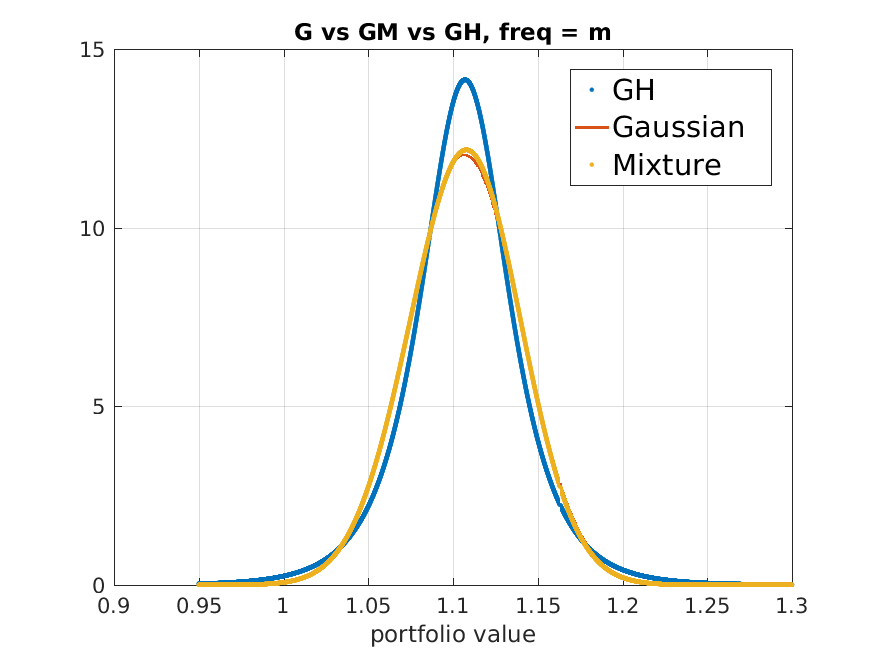
\includegraphics[width=0.5\textwidth]{GvsGMvsGHm.png}}
	\hfill
	\subfloat[]{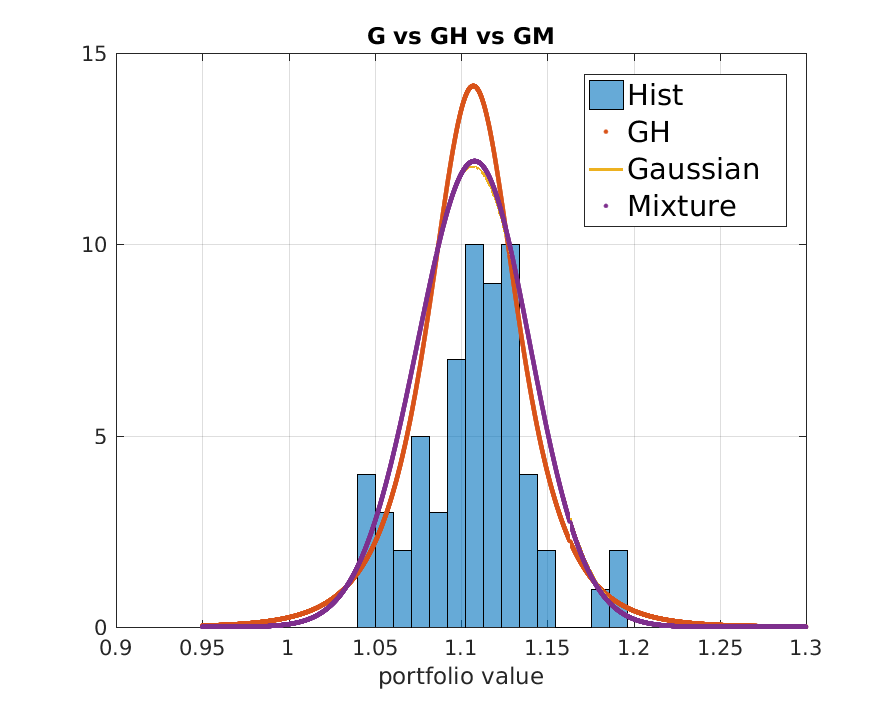
\includegraphics[width=0.5\textwidth]{histm.png}}
	\hfill
	\subfloat[]{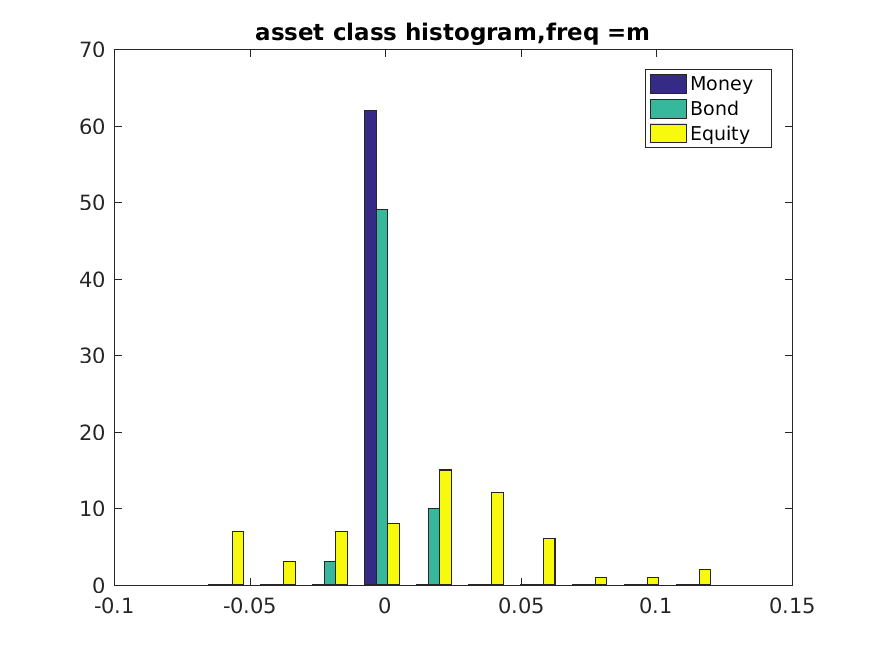
\includegraphics[width=0.5\textwidth]{histReturnsm.png}}
	\caption{}
\end{figure}

\begin{center}
	\begin{tabular}{|c || c| c| c| c|} 
		\hline
		freq = m & G & GM & GH  & Estimated\\ [0.5ex] 
		\hline\hline
		Skewness & 0 & -0.039858 & -0.040361 & 0.15053 \\ 
		\hline
		Kurtosis & 3 & 2.7604 & 5.4111 & 3.1827\\
		\hline
		LogL & 736.2216 & 755.507 & 743.3431 \\
		\hline
		AIC &  & -1473.0141 & -1460.6862 \\[1ex] 
		\hline
	\end{tabular}
\end{center}
\subsubsection{weekly frequency}


\begin{figure}[H]
	\centering
	\subfloat[]{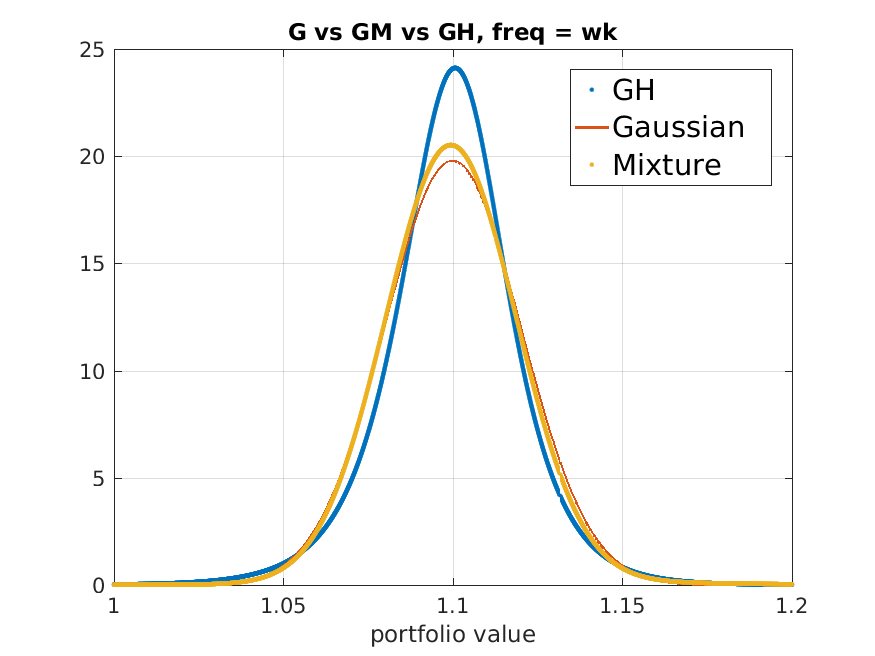
\includegraphics[width=0.5\textwidth]{GvsGMvsGHwk.png}}
	\hfill
	\subfloat[]{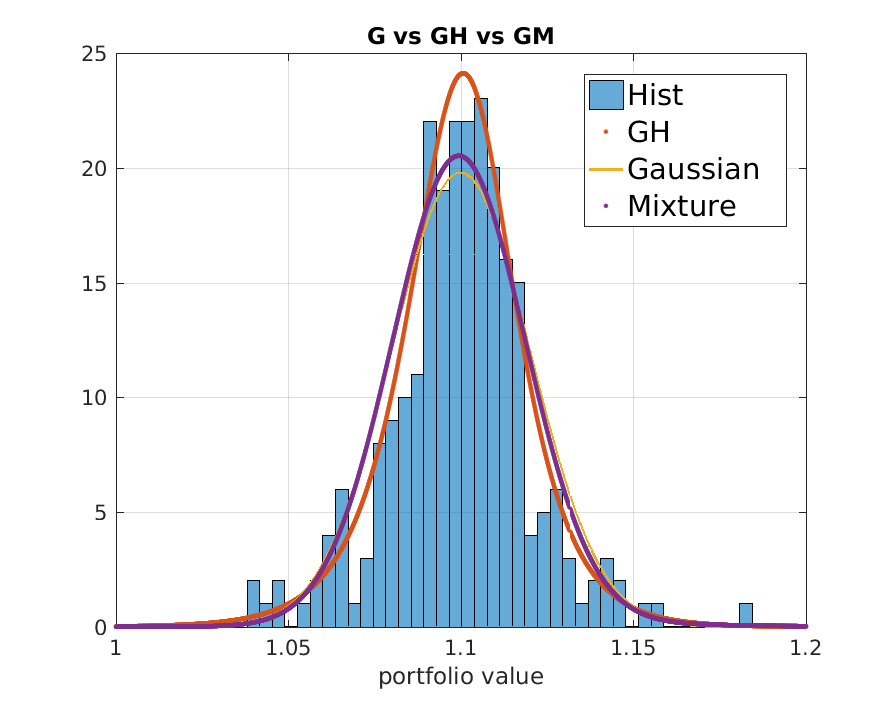
\includegraphics[width=0.5\textwidth]{histwk.png}}
	\hfill
	\subfloat[]{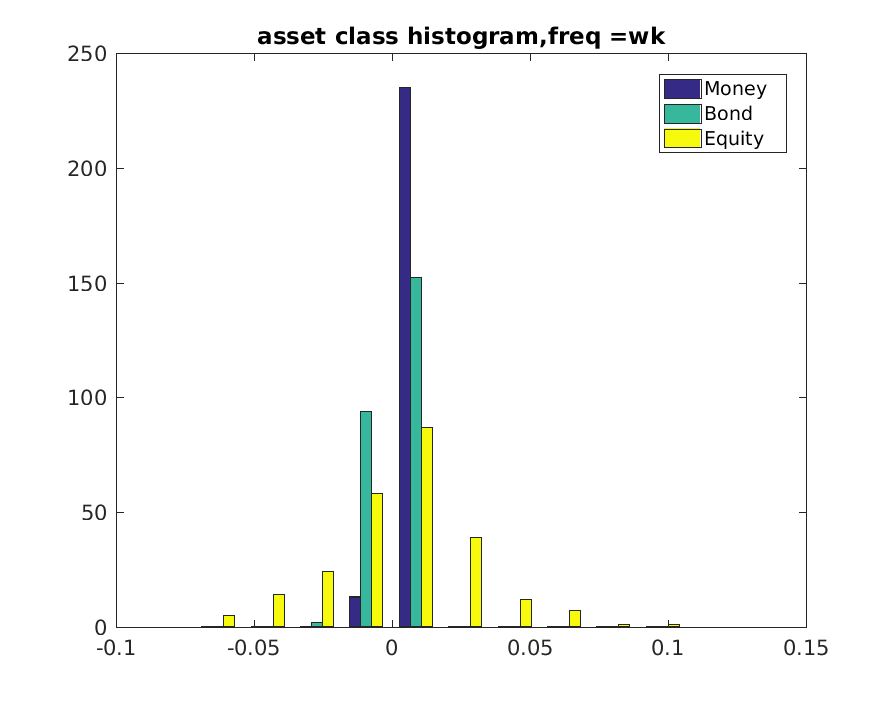
\includegraphics[width=0.5\textwidth]{histReturnswk.png}}
	\caption{}
\end{figure}

\begin{center}
	\begin{tabular}{|c || c| c| c| c|} 
		\hline
		 freq = wk & G & GM & GH & Estimated\\ [0.5ex] 
		\hline\hline
		Skewness & 0 & 0.24234 & -0.16078 & 0.026168\\ 
		\hline
		Kurtosis & 3 & 4.1407 & 4.8293 & 4.6452\\
		\hline
		LogL & 3295.6076 & 3346.4078 & 3335.7617 \\
		\hline
		AIC &  & -6654.8156 & -6645.5235 \\[1ex] 
		\hline
	\end{tabular}
\end{center}


\subsubsection{daily frequency}

\begin{figure}[H]
	\centering
	\subfloat[]{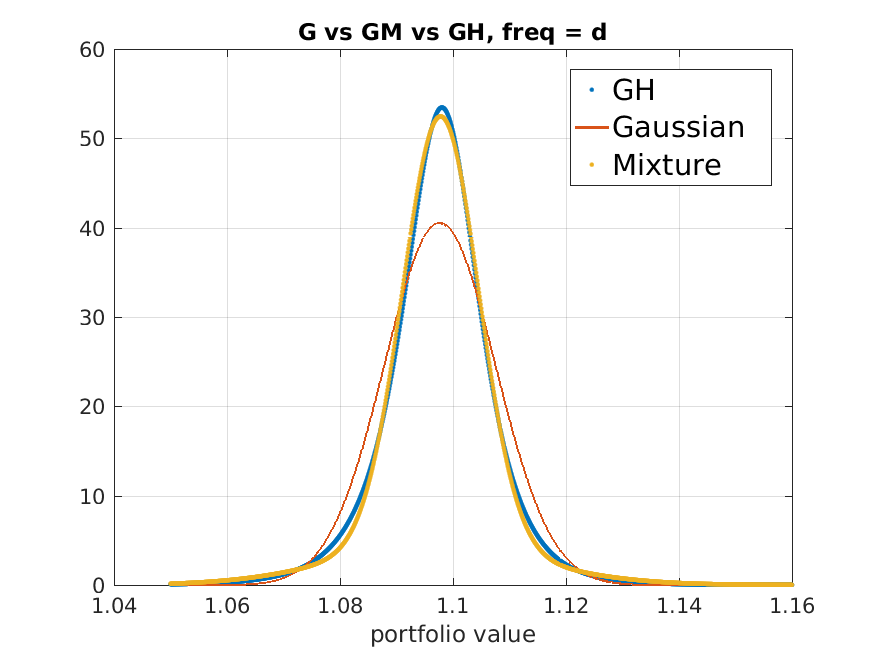
\includegraphics[width=0.5\textwidth]{GvsGMvsGHd.png}}
	\hfill
	\subfloat[]{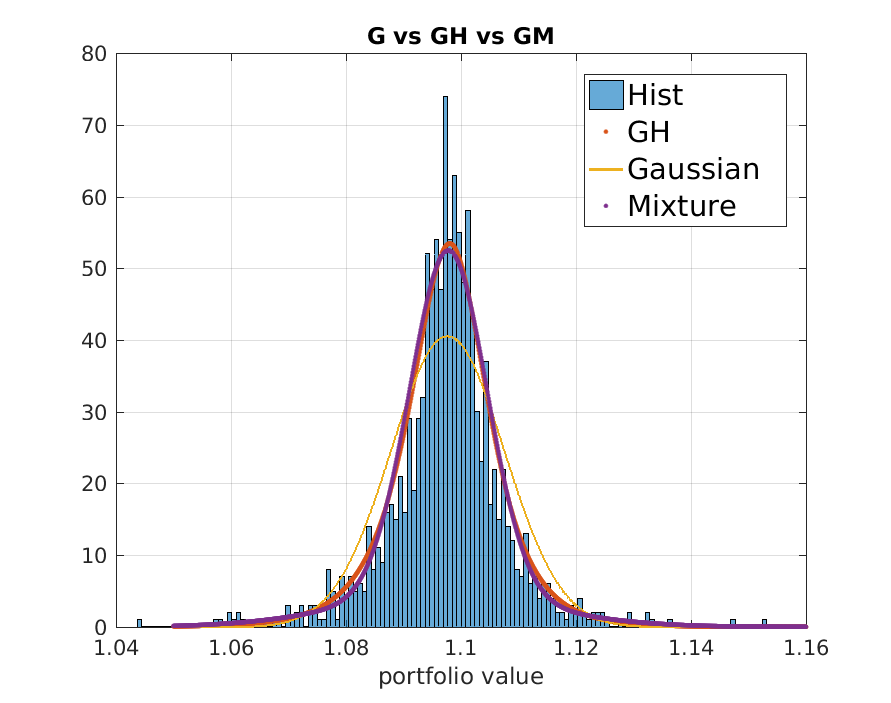
\includegraphics[width=0.5\textwidth]{histd.png}}
	\hfill
	\subfloat[]{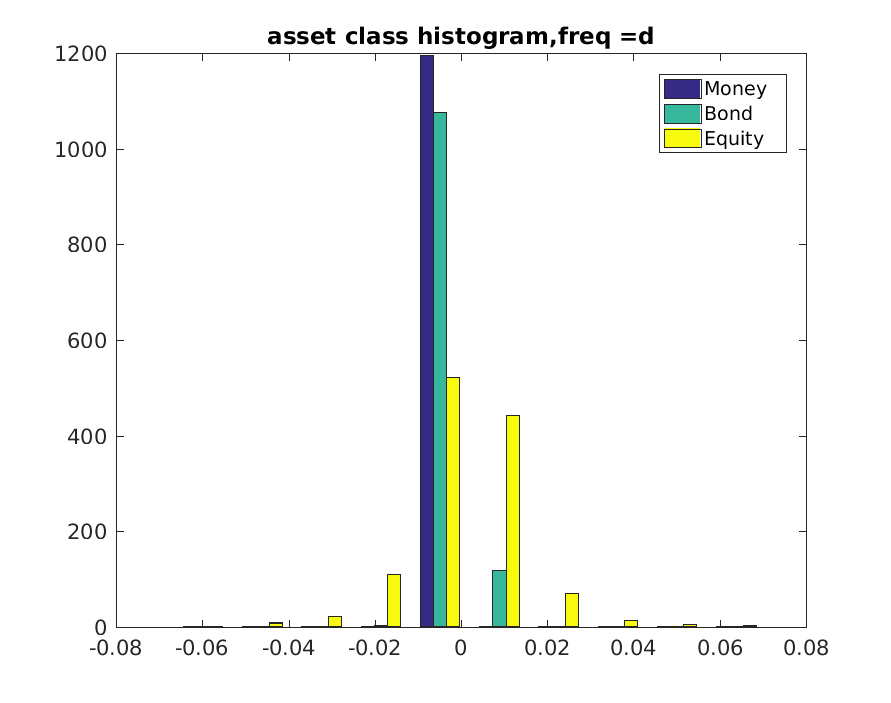
\includegraphics[width=0.5\textwidth]{histReturnsd.png}}
	\caption{}
\end{figure}
\begin{center}
	\begin{tabular}{|c || c| c| c| c|} 
		\hline
		freq = d & G & GM & GH & Estimated \\ [0.5ex] 
		\hline\hline
		Skewness & 0 & -0.16716 & -0.21467 & -0.1301\\ 
		\hline
		Kurtosis & 3 & 6.6815 & 5.6486 & 6.9324\\
		\hline
		LogL & 17959.9792 & 18202.8555 & 18219.1673 \\
		\hline
		AIC &  & -36367.7109 & -36412.3345 \\[1ex] 
		\hline
	\end{tabular}
\end{center}


\subsection{allocation maps}
\subsubsection{Gaussian Mixture}
\begin{figure}[H]
	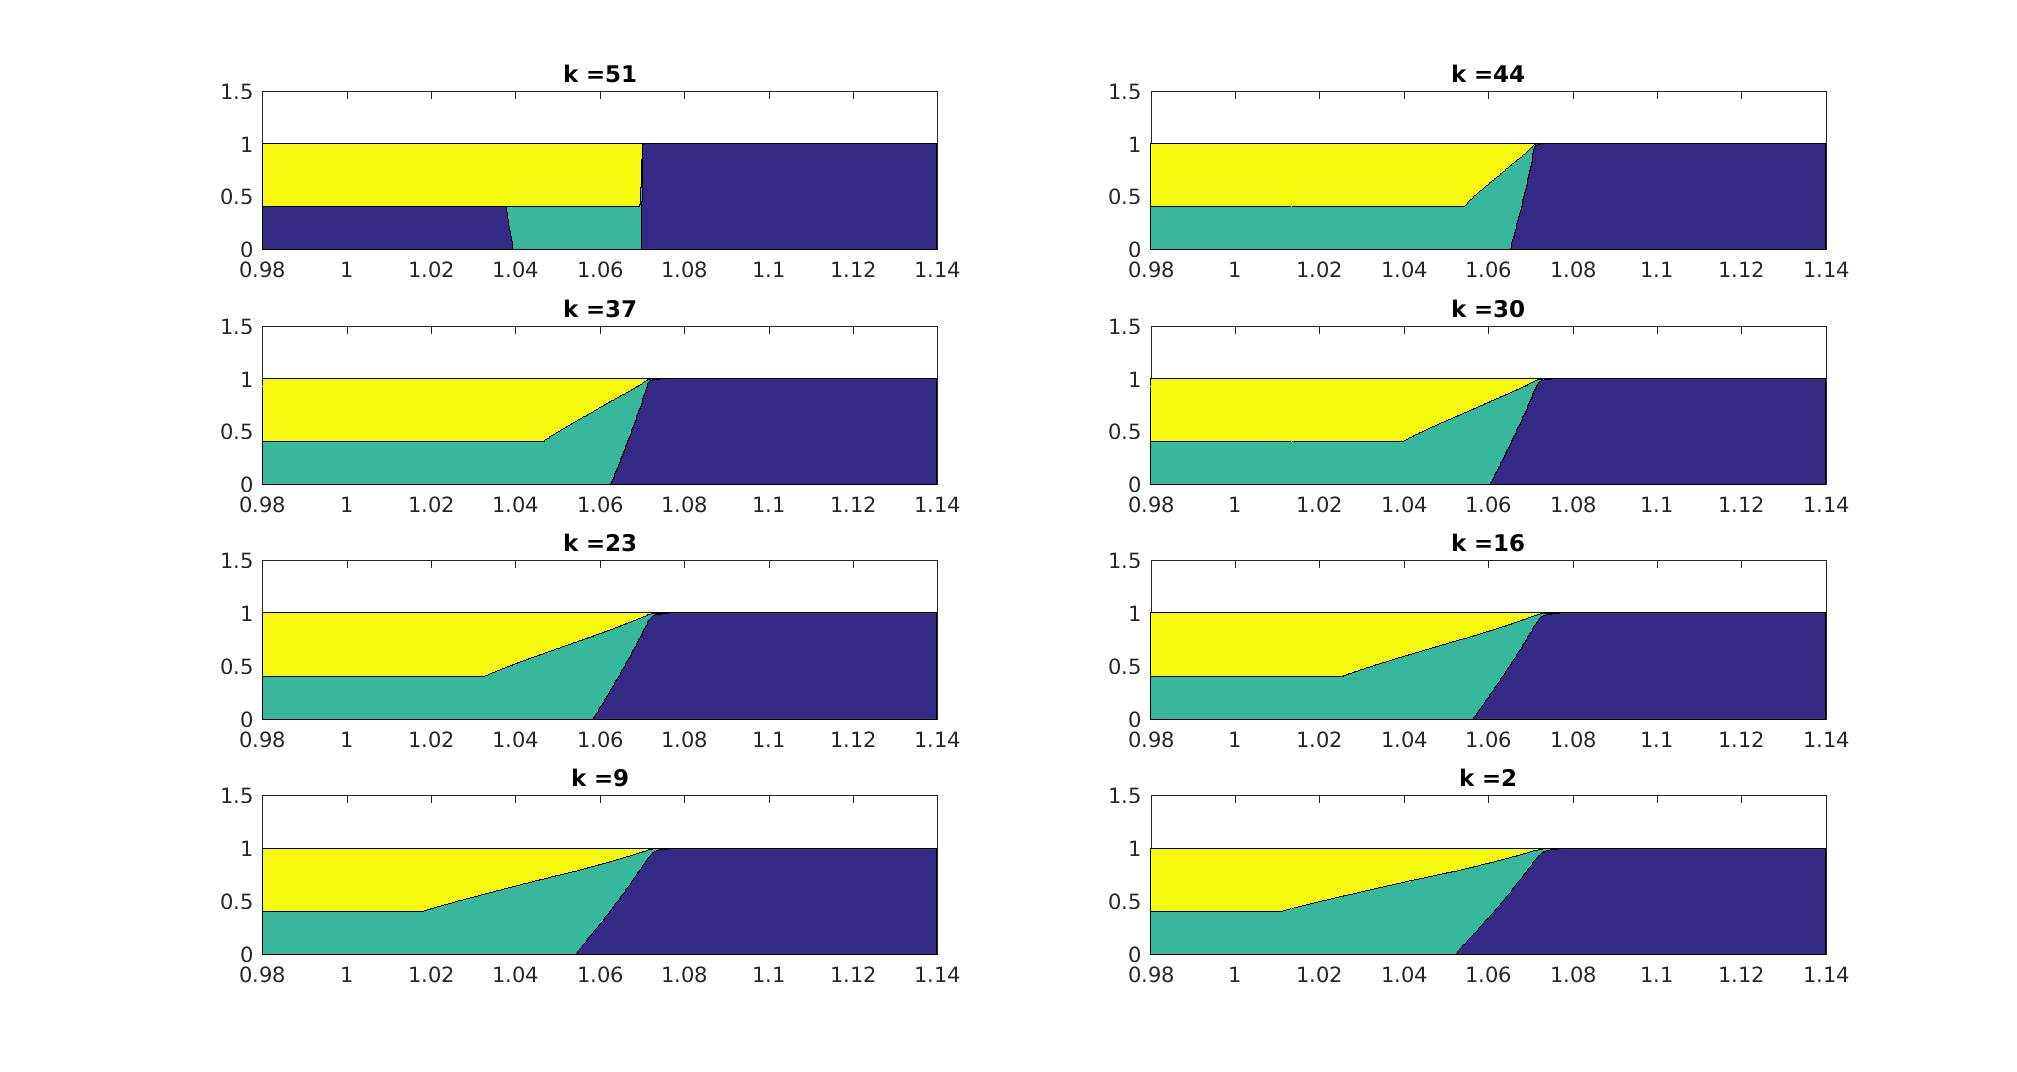
\includegraphics[width=\textwidth]{Mixture.png}
\end{figure}

\subsubsection{Generalized Hyperbolic}



\section{problems}
\begin{figure}[H]
	\centering
	\subfloat[]{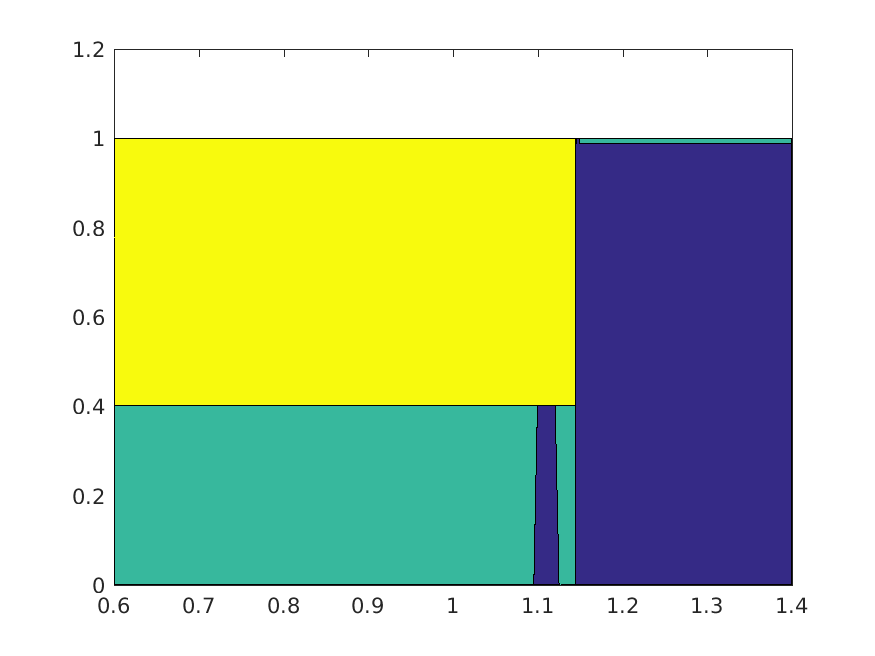
\includegraphics[width=0.5\textwidth]{error1.png}}
	\hfill
	\subfloat[]{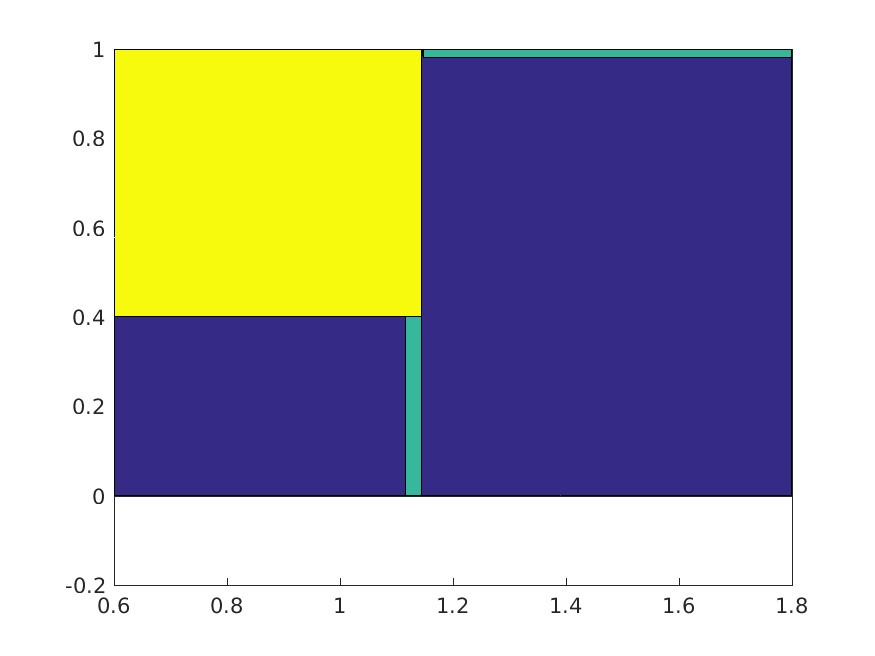
\includegraphics[width=0.5\textwidth]{error2.png}}
	\caption{k = N}
\end{figure}

\end{document}
